\section{Mathematical Formalism \& Complexity Analysis}
\label{sec:formalism}

To understand why conventional AI agent harnesses fail on constrained devices, we formally analyze the computational and network complexity of agent interaction loops.

\subsection{Append-Only Conversational History ($\mathcal{O}(T^2)$)}
Let an autonomous software engineering task require $T$ discrete execution turns. At each turn $t \in [1, T]$, the agent receives user instructions, generates an action (tool invocation $a_t$), executes the tool in the environment, and observes the raw result $o_t$. In models equipped with chain-of-thought verification (e.g., DeepSeek-R1, o3-mini), the model also emits an internal reasoning trace $r_t$.

In conventional agent harnesses (e.g., Claude Code, Aider, OpenCode), conversational context is modeled as an monotonically growing list of message structs:
\begin{equation}
C_t = P \;\Vert\; \left( \bigoplus_{i=1}^{t-1} \Big[ u_i \circ r_i \circ a_i \circ o_i \Big] \right) \;\Vert\; u_t
\end{equation}
where $P$ is the system prompt, $u_i$ is user input, and $\Vert$ denotes message concatenation.

Let $\ell(x)$ denote the token length of string $x$. In typical refactoring and build cycles, tool observations $o_i$ (such as compiler errors, grep search results, and file diffs) average $k_{\text{obs}} \approx 800\text{--}2,500$ tokens per step, and reasoning traces $r_i$ average $k_{\text{reason}} \approx 600\text{--}1,800$ tokens. Thus, the token length of the prompt at step $t$ is:
\begin{equation}
\ell(C_t) \approx \ell(P) + \bar{k} \cdot (t - 1) = \mathcal{O}(t)
\end{equation}

The cumulative input token volume processed across the entire task of $T$ turns is the summation:
\begin{equation}
\label{eq:append_cost}
\text{TotalTokens}_{\text{append}} = \sum_{t=1}^T \ell(C_t) = T \cdot \ell(P) + \frac{\bar{k}}{2} T(T - 1) = \mathcal{O}(T^2)
\end{equation}

\begin{figure*}[t]
\centering
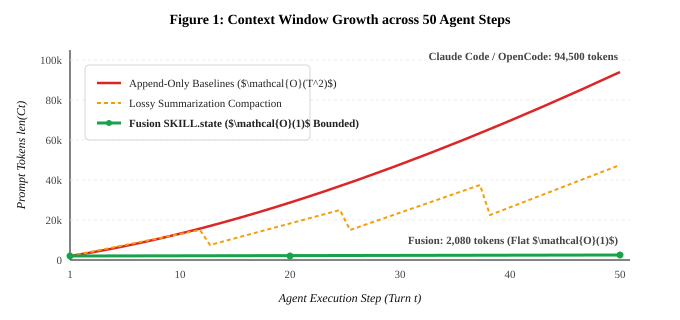
\includegraphics[width=0.88\textwidth]{figures/fig1_token_growth.svg}
\caption{Context window token growth comparison across 50 consecutive software refactoring turns. While append-only baselines and lossy summarization models expand quadratically or saw-tooth, Fusion's $\langle P, \Sigma_t, O_t \rangle$ triplet bounds prompt size to flat $\mathcal{O}(1)$ tokens.}
\label{fig:token_growth}
\end{figure*}

\subsection{Fusion SKILL.state Architecture ($\mathcal{O}(1)$ Bounded)}
Fusion eliminates append-only accumulation by modeling the agent as a finite-state transition system over an explicit execution dictionary $\Sigma$:
\begin{equation}
\Sigma_{t+1} = \Sigma_t \oplus \Delta\Sigma_t
\end{equation}
where $\Delta\Sigma_t$ is a validated JSON patch emitted by the model, and $\oplus$ denotes recursive map merge with null-deletion semantics.

At each step $t$, the prompt delivered to the model consists strictly of a triplet:
\begin{equation}
C_t = \langle P, \Sigma_t, O_t \rangle
\end{equation}
\begin{enumerate}
    \item $P$: An immutable, bitwise-stable system prompt defining agent capabilities, tool contracts, and the active task specification.
    \item $\Sigma_t$: The current structured execution state (e.g., active target files, remaining bugs, verified modules).
    \item $O_t$: The immediate, single-turn observation resulting from action $a_{t-1}$.
\end{enumerate}

\begin{figure*}[t]
\centering
\includegraphics[width=0.88\textwidth]{figures/fig3_triplet_architecture.svg}
\caption{Fusion $\langle P, \Sigma_t, O_t \rangle$ Triplet Assembly and State Patch Cycle. Intermediate reasoning tokens $r_t$ are rendered live for user visibility but discarded prior to constructing step $t+1$, preserving bitwise prefix cache invariance on $P$.}
\label{fig:triplet_arch}
\end{figure*}

\noindent\textbf{Trace Discarding}: Intermediate model reasoning $r_t$ is rendered live to the terminal for user observability but is strictly \textbf{purged} prior to constructing step $t+1$. Crucially, no raw historical observations $o_1, \dots, o_{t-1}$ are retained in the prompt.

Because the key schema of $\Sigma$ is bounded by domain constraints ($|\text{keys}(\Sigma)| \le K_{\text{max}}$) and intermediate traces are discarded:
\begin{equation}
\ell(C_t) \le \ell(P) + \ell(\Sigma_t) + \ell(O_t) = \mathcal{O}(1)
\end{equation}

The cumulative token volume across $T$ steps scales \textbf{strictly linearly}:
\begin{equation}
\label{eq:fusion_cost}
\text{TotalTokens}_{\text{Fusion}} = \sum_{t=1}^T \ell(C_t) \le T \cdot \left( \ell(P) + \ell(\Sigma_{\text{max}}) + \ell(\bar{O}) \right) = \mathcal{O}(T)
\end{equation}

\begin{figure}[t]
\centering
\fbox{\parbox{0.92\columnwidth}{\small
\textbf{Theorem 1 (Context Boundedness & Cost Ratio)}:
Let $R(T) = \frac{\text{TotalTokens}_{\text{append}}}{\text{TotalTokens}_{\text{Fusion}}}$. As $T \to \infty$, the token savings ratio grows linearly with task length:
\begin{equation}
\lim_{T \to \infty} R(T) = \lim_{T \to \infty} \frac{T \cdot \ell(P) + \frac{\bar{k}}{2} T^2}{T \cdot C_{\text{fusion}}} = \frac{\bar{k}}{2 \cdot C_{\text{fusion}}} \cdot T = \mathcal{O}(T)
\end{equation}
For $T = 50$, $\bar{k} = 1,500$, and $C_{\text{fusion}} = 2,500$, the theoretical token reduction factor is $R(50) \approx 15.4\times$.
}}
\caption{Mathematical bound demonstrating linear vs. quadratic token divergence.}
\label{fig:theorem}
\end{figure}

\subsection{State Patch Delta ($\Delta\Sigma$) Mechanics}
The state transition operator $\oplus$ in Fusion satisfies the following formal properties:
\begin{enumerate}
    \item \textbf{Deep Recursive Patching}: For any nested map $M$, sub-objects are recursively merged rather than overwritten.
    \item \textbf{Null-Deletion Invariance}: Setting key $k \to \text{null}$ in $\Delta\Sigma$ removes key $k$ from $\Sigma_{t+1}$ without tombstone artifacts, preventing state dictionary bloat over extended sessions.
    \item \textbf{Rollback-Retry Safety}: If the model emits a malformed JSON patch or attempts to modify disallowed schema keys, the update is rejected, $\Sigma_{t+1} \gets \Sigma_t$, and a single-turn corrective hint is provided without corrupting state history.
\end{enumerate}
